\normalfalse \difficilefalse \tdifficiletrue
\correctionfalse

%\UPSTIidClasse{11} % 11 sup, 12 spé
%\newcommand{\UPSTIidClasse}{12}

\exer{Système 4 barres $\star\star$ \label{C2:09:17}} 
\setcounter{question}{0}\UPSTIcompetence[2]{C2-09}
\index{Compétence C2-09}
\index{TEC}
\index{Théorème de l'énergie cinétique}
\index{Système 4 barres}
\index{Portail}
\ifcorrection
\else
\marginnote{\textbf{Pas de corrigé pour cet exercice.}}
\fi

\ifprof
\else
On a : 
%\begin{multicols}{2}
\begin{itemize}
\item $\vect{OA} = a \vx{1}-f \vy{1}$ avec $a=\SI{355}{mm}$ et $f=\SI{13}{mm}$;
\item $\vect{AB} = b \vx{2}$ avec $b=\SI{280}{mm}$;
\item $\vect{BC} = -c \vx{3}$ avec $c=\SI{280}{mm}$;
\item $\vect{OC} = -d \vx{0}-e\vy{0}$ avec $d=\SI{89,5}{mm}$ et $e=\SI{160}{mm}$.
\end{itemize}
De plus, on note :
\begin{itemize}
\item $G_1$ le centre d'inertie du solide \textbf{1} tel que $\vect{OG_1}=L \vx{1}$, $m_1$ sa masse et $\inertie{G_1}{1}=\matinertie{A_1}{B_1}{C_1}{0}{0}{0}{\rep{1}}$ sa matrice d'inertie;
\item $G_2$ le centre d'inertie du solide \textbf{2} tel que $\vect{AG_2}=\dfrac{b}{2}\vx{2}$, $m_2$ sa masse et $\inertie{G_2}{2}=\matinertie{A_2}{B_2}{C_2}{0}{0}{0}{\rep{2}}$ sa matrice d'inertie;
\item $G_3$ le centre d'inertie du solide \textbf{3} tel que $\vect{CG_3}=\dfrac{c}{2}\vx{3}$, $m_3$ sa masse et $\inertie{G_3}{3}=\matinertie{A_3}{B_3}{C_3}{0}{0}{0}{\rep{3}}$ sa matrice d'inertie.
\end{itemize}
On note $C_m\vk{0}$ le couple moteur agissant sur le solide \textbf{1}. L'accélération de la pesanteur est donnée par $\vect{g}=-g\vz{0}$.
%\end{multicols}
%a,b,c,d,e,ff = 355,280,280,89.5,160,13

\begin{center}
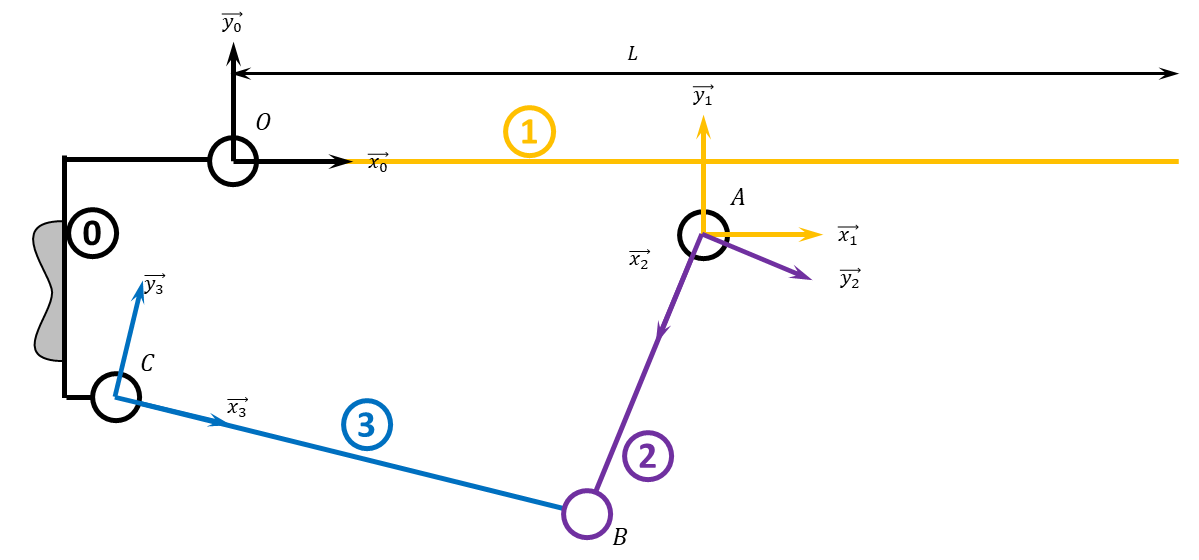
\includegraphics[width=\linewidth]{17_01}

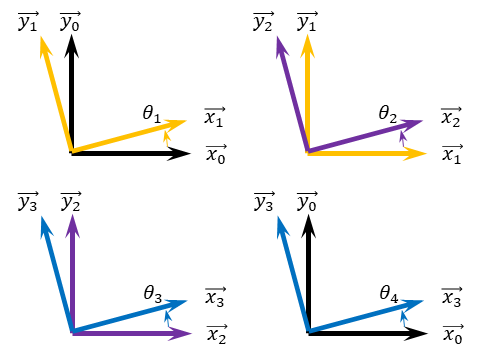
\includegraphics[width=\linewidth]{17_02}
\end{center}
\fi
On rappelle que la loi entrée sortie est donnée par la relation *** établie à l'exercice \ref{C2:06:17}.

\question{Tracer le graphe d'analyse en indiquant l'ensemble des actions mécaniques agissant sur les différents solides.}
\ifprof
\else
\fi

\question{Déterminer l'ensemble des puissances intérieures à l'ensemble \textbf{1+2+3}.}
\ifprof
\else
\fi

\question{Déterminer l'ensemble des puissances extérieures à l'ensemble \textbf{1+2+3}.}
\ifprof
\else
\fi

\question{Déterminer $\ec{1+2+3}{0}$.}
\ifprof
\else
\fi

\question{Déterminer la loi de mouvement en appliquant le théorème de l'énergie cinétique.}
\ifprof
\else
\fi


\ifprof
\else
\begin{flushright}
\footnotesize{Corrigé  voir \ref{C2:09:17}.}
\end{flushright}%
\fi